\documentclass{beamer}
\usetheme{Boadilla}

\usepackage{mathtools}
\usepackage{graphicx}
\usepackage{tikz}

\graphicspath{ {./images/} }

\newcommand{\cntxt}{\ \mathrm{context}}
\newcommand{\typ}{\ \mathrm{type}}
\newcommand{\N}{\mathbb{N}}
\newcommand{\app}[2]{App_{[x:\sigma]\tau}(#1, #2)}
\newcommand{\pair}[2]{Pair_{[x:\sigma]\tau}(#1, #2)}
\newcommand{\R}[2]{\mathrm{R}_{[z:\Sigma x:\sigma.\tau]\rho}^{\Sigma}(#1, #2)}
\newcommand{\RN}[3]{\mathrm{R}_{[n: \N]\sigma}^{\N}(#1, #2, #3)}
\newcommand{\C}{Comp}
\newcommand{\Intro}{Intro}
\newcommand{\F}{Form}
\newcommand{\E}{Elim}
\newcommand\defeq{\stackrel{\mathclap{\normalfont\mbox{def}}}{\ =\ }}
\newcommand{\Id}[2]{Id_\sigma(#1,#2)}
\newcommand{\Refl}[1]{Refl_\sigma(#1)}
\newcommand{\RID}[4]{\mathrm{R}_{[x:\sigma,y:\sigma,p:Id_\sigma(x,y)]\tau}^{Id}(#1, #2, #3, #4)}
\newcommand{\bn}{[n:\N,x:\sigma]}
\newcommand{\bi}{[z:\sigma]}


\title{Dependant Types}
\subtitle{Initiation to research}
\author{Louis Milhaud}
\institute{Université Paris Saclay}
\date{\today}

\begin{document}
    \begin{frame}
        \titlepage
    \end{frame}
    \begin{frame}
        \frametitle{Outline}
        \tableofcontents
    \end{frame}
    \section{Introduction}
    \subsection{History}
    \begin{frame}
        \frametitle{History}
        \begin{itemize}
            \item[-] 1972: System F, G. Huet
            \item[-] 1975: \underline{Intuitionnistic Type Theory}, P. Martin-Lof
            \item[-] 1986: Nuprl System
            \item[-] 1988: Calculus of Construction, T. Coquand  
            \item[-] 1989: Coq
            \item[-] 1997: \underline{Syntax \& Semantics of Dependant Type Theory}, M. Hofmann 
        \end{itemize}
    \end{frame}
    \subsection{Definition}
    \begin{frame}
        \frametitle{Definition}
        A dependant type is a family of types varying on the elements of another type.\\
        \vspace{20pt}
        \underline{Example:}\\
        $$Vec_\sigma(M),\quad M:\N $$
        with the following objects:
        \begin{itemize}
            \item $nil_\sigma : Vec_\sigma(0)$
            \item $Cons_\sigma(U, V) : Vec_\sigma(Succ(M))$ 
        \end{itemize}
        with $ U : \sigma\ \text{ and } V : Vec_\sigma(M)$
    \end{frame}
    \subsection{Judgments \& Equality}
    \begin{frame}
        \frametitle{Judgments}
        \begin{align}
            &\vdash \Gamma \cntxt &\Gamma \text{ is a valid context}\\
            \Gamma &\vdash \sigma \typ &\sigma \text{ is a type in context $\Gamma$}\\
            \Gamma &\vdash M : \sigma &M\text{ is a term of type $\sigma$ in context $\Gamma$}\\
            &\vdash \Gamma = \Delta \cntxt &\text{$\Gamma$ and $\Delta$ are definitionaly equal contexts}\\
            \Gamma &\vdash \sigma = \tau &\text{$\sigma$ and $\tau$ are def. equal types in context $\Gamma$}\\
            \Gamma &\vdash M = N : \sigma &M\text{ and }N\text{ are def. equal terms of $\sigma$ in $\Gamma$}
        \end{align}
    \end{frame}
    \begin{frame}
        \frametitle{Definitional Equality}
        \underline{Definitional Equality (Per Martin-Lof):}\\
        \vspace{10pt}
        \emph{"Definitional equality is intensional equality, or equality of meaning."}\\
        \vspace{10pt}
        This equality defines an equivalence relation:
        $$\frac{\vdash \Gamma \cntxt}{\vdash \Gamma = \Gamma \cntxt}\qquad \frac{\vdash \Gamma = \Delta \cntxt}{\vdash \Delta = \Gamma \cntxt}$$
        $$\frac{\vdash \Gamma = \Theta \cntxt \vdash \Theta = \Delta \cntxt}{\vdash \Gamma = \Delta \cntxt}$$
        With the same rules for types and terms.
    \end{frame}
    \begin{frame}
        \frametitle{Notions of Equality}
        \underline{Three notions of equality:}
        \begin{itemize}
            \item[-] Judgmental equality
            $$\frac{\Gamma \vdash \N \typ}{\Gamma \vdash 1:\N} \qquad \frac{\Gamma \vdash \N \typ}{\Gamma \vdash 1 = Suc(0):\N}$$
            \item[-] Typal equality
            $$\frac{\Gamma \vdash \N \typ}{\Gamma \vdash 1:\N} \qquad \frac{\Gamma \vdash \N \typ}{\Gamma \vdash \delta_1:1 =_{\N} Suc(0)}$$
            \item[-] Propositional equality
            $$\frac{\Gamma \vdash \N \typ}{\Gamma \vdash 1:\N} \qquad \frac{\Gamma \vdash \N \typ}{\Gamma \vdash 1 =_{\N} Suc(0) \; \mathrm{true}}$$
        \end{itemize}
    \end{frame}
    \subsection{Basic rules}
    \begin{frame}
        \frametitle{Basic rules 1}
        \underline{Rules for context formation:}
        $$\frac{}{\vdash \diamond \cntxt} \qquad \frac{\Gamma \vdash \sigma \typ}{\vdash \Gamma, x: \sigma \cntxt}$$
        $$\frac{\Gamma = \Delta \cntxt \quad \Gamma \vdash \sigma = \tau \typ}{\vdash \Gamma, x: \sigma = \Delta, y:\tau \cntxt}$$
        \underline{Variable Rule:}
        $$\frac{\vdash \Gamma, x: \sigma, \Delta \cntxt}{\Gamma, x:\sigma,\Delta\vdash x : \sigma}$$
    \end{frame}
    \begin{frame}
        \frametitle{Basic rules 2}
        \underline{Rules for typing and definitional equality:}
        $$\frac{\Gamma \vdash M : \sigma \quad \vdash \Gamma = \Delta \cntxt \quad \Gamma \vdash \sigma = \tau \typ}{\Delta \vdash M : \tau}$$
        $$\frac{\vdash \Gamma = \Delta \cntxt \quad \Gamma \vdash \sigma \typ}{\Delta \vdash \sigma \typ}$$
        \underline{Weakening and substitution Rules:}
        $$\frac{\Gamma, \Delta \vdash \mathcal{J} \quad \Gamma \vdash \rho \typ}{\Gamma, x: \rho, \Delta\vdash \mathcal{J}}$$
        $$\frac{\Gamma,x:\rho,\Delta \vdash \mathcal{J}\quad \Gamma \vdash U: \rho}{\Gamma,\Delta[U/x]\vdash \mathcal{J}[U/x]}$$
    \end{frame}
    \section{Type formers}
    \subsection{$\prod$-type}
    \begin{frame}
        \frametitle{$\prod$-type}
        \begin{itemize}
            \item Called dependant product, dependant function space, $\pi$-type...
            \item Type former for the functions which the return type depends on the element of the entry type.
            \item \underline{Set-theoretic equivalent:}\\
            Cartesian product over a family of sets: $\Pi_{i\in I}B_i$
            \item \underline{type former rules:} type formation, term introduction, term elimination, computation rule and an optional uniqueness rule. And type formers are preserved by definitional equality.
        \end{itemize}
    \end{frame}
    \begin{frame}
        \frametitle{Rules}
        $$\frac{\Gamma \vdash \sigma \typ \quad \Gamma,x:\sigma\vdash \tau \typ}{\Gamma \vdash \Pi x:\sigma.\tau \typ}\F$$
        \vspace{10pt}
        $$\frac{\Gamma, x:\sigma \vdash M : \tau}{\Gamma \vdash \lambda x:\sigma.M^\tau : \Pi x:\sigma.\tau}\Intro$$
        \vspace{10pt}
        $$\frac{\Gamma \vdash \lambda x:\sigma.M^\tau:\Pi x:\sigma.\tau \quad \Gamma \vdash N:\sigma}{\Gamma \vdash \app{\lambda x:\sigma.M^{\tau}}{N} = M[N/x]:\tau[N/x]}\C$$
        \vspace{10pt}
        $$\frac{\Gamma \vdash M : \Pi x: \sigma . \tau \quad \Gamma \vdash N: \sigma}{\Gamma \vdash \app{M}{N}: \tau[N/x]}\E$$
    \end{frame}
    \subsection{$\sum$-type}
    \begin{frame}
        \frametitle{$\sum$-type}
        \begin{itemize}
            \item Type former for pairs which the second element type depends on the first element.
            \item \underline{Set-theoretic equivalent:}\\
            Disjoint union over a family of sets: $\Sigma_{i\in I}B_i \defeq \{(i,b)|i \in I \wedge b \in B_i\}$
            \item $\pi_1 \defeq \R{[x:\sigma,y:\tau]x}{M}:\sigma$
            \item $\pi_2 \defeq \mathrm{R}^\Sigma_[z:\Sigma x:\sigma.\tau]\tau[z.1/x]([x:\sigma,y:\tau]y, M):\tau[M.1]$
        \end{itemize}
    \end{frame}
    \begin{frame}
        \frametitle{Rules}
        $$\frac{\Gamma \vdash \sigma \typ \quad \Gamma,x:\sigma\vdash \tau \typ}{\Gamma\vdash \Sigma x:\sigma.\tau \typ}\F$$
        $$\frac{\Gamma \vdash M : \sigma\quad \Gamma \vdash N : \tau[M/x]}{\Gamma \vdash \pair{M}{N} : \Sigma x:\sigma.\tau}\Intro$$
        $$\frac{\Gamma \vdash \R{[x:\sigma,y:\tau]H}{\pair{M}{N}:\rho[\pair{}{}/z]}}{\Gamma \vdash \R{[x:\sigma,y:\tau]H}{\pair{M}{N}}}\C$$
        $$=H[M/x,N/y]:\rho[\pair{}{}/z].$$
        $$\Gamma,z:\Sigma x:\sigma.\tau \vdash \rho \typ$$
        $$\Gamma,x:\sigma,y:\tau\vdash H:\rho [\pair{x}{y}/z]$$
        $$\frac{\quad \Gamma \vdash M : \Sigma x:\sigma.\tau}{\Gamma \vdash \R{[x:\sigma.y:\tau]H}{M}:\rho[M/z]}\E$$
    \end{frame}
    \subsection{Naturals}
    \begin{frame}
        \frametitle{Naturals}
        Naturals are as always inductively defined, thus we have the two following objects:
        $$0 \text{ and } Suc(M) \text{ with } M:\N$$
        \vspace{10pt}
        Then we can define operations like addition:
        $$M + N \defeq \RN{N}{[n:\N, x:\N]Suc(x)}{M}:\N$$
    \end{frame}
    \begin{frame}
        \frametitle{Rules}
        $$\frac{\vdash \Gamma \cntxt}{\Gamma \vdash \N \typ}\F \frac{\vdash \Gamma \cntxt}{\Gamma \vdash 0 : \N}\& \frac{\Gamma \vdash M : \N}{\Gamma \vdash Suc(M):\N}\Intro$$
        $$\Gamma,n:\N\vdash\sigma\typ$$
        $$\Gamma\vdash H_z : \sigma[0/n]$$
        $$\Gamma,n:\N,x:\sigma\vdash H_s : \sigma[Suc(n)/n]$$
        $$\frac{\Gamma\vdash M: \N}{\Gamma\vdash\RN{H_z}{[n:\N,x:\sigma]H_s}{M}:\sigma[M/n]}\E$$
        $$\frac{\Gamma \vdash \RN{H_z}{\bn H_s}{0} : \sigma[0/n]}{\Gamma \vdash \RN{H_z}{\bn H_s}{0} = H_z: \sigma[0/n]}\C$$
        $$\frac{\Gamma \vdash \RN{H_z}{\bn H_s}{Suc(M)} : \sigma[Suc(M)/n]}{\Gamma \vdash \RN{H_z}{\bn H_s}{Suc(M)} =}\C$$
        $$ H_s[M/n,\RN{H_z}{\bn H_s}{M}/x]:\sigma[Suc(M)/n]$$
    \end{frame}
    \subsection{Identity types}
    \begin{frame}
        \frametitle{Identity types}
        \begin{itemize}
            \item Type former for typal equality
            \item Enables equality reasonning inside type theory
            \item $\Refl{M} : \Id{M}{M}$ with $M : \sigma$
            \item We can deduce other properties of typal equality like symmetry, transitivity, Leibniz principle thanks to the elimination rule.
        \end{itemize}
    \end{frame}
    \begin{frame}
        \frametitle{Rules}
        $$\frac{\Gamma\vdash M:\sigma \quad \Gamma\vdash N:\sigma}{\Gamma \vdash \Id{M}{N} \typ}\F$$
        $$\frac{\Gamma\vdash M:\sigma}{\Gamma\vdash\Refl{M}:\Id{M}{M}}\Intro$$
        $$\Gamma\vdash\sigma\typ\quad\Gamma\vdash M:\sigma\quad\Gamma\vdash N:\sigma$$
        $$\Gamma, x:\sigma,y:\sigma,p:\Id{x}{y}\vdash\tau\typ$$
        $$\Gamma,z:\sigma\vdash H:\tau[z/x,z/y,\Refl{z}/p]$$
        $$\frac{\Gamma\vdash P:\Id{M}{N}}{\Gamma\vdash\RID{[z:\sigma]H}{M}{N}{P}:\tau[M/x,N/y,P/p]}\E$$
        $$\frac{\Gamma \vdash \RID{\bi H}{M}{M}{\Refl{M}}:\tau[M/x,M/y,\Refl{M}/p]}{\Gamma \vdash\ idem = H[M/z]:\tau[M/x,M/y,\Refl{M}/p]}$$$\C$
    \end{frame}
    \subsection{Universes}
    \begin{frame}
        \frametitle{Universes}    
    \end{frame}
    \begin{frame}
        \frametitle{Rules}
        $$\frac{\vdash \Gamma \cntxt}{\Gamma \vdash U \typ}\quad\frac{\Gamma \vdash M:U}{\Gamma\vdash El(M)\typ}$$
    \end{frame}
    \section{Categoretical Semantics}
    \begin{frame}
        \frametitle{Categoretical Semantics: the idea}
        \begin{itemize}
            \item Let $A \typ$ interprets as an object in some category $\mathcal{C}$
            \item Let $x: A \vdash B \typ$ interprets as a morphism $B \rightarrow A$ in $\mathcal{C}$
            \item Let $x: A \vdash B \typ$ interprets as an object in the slice category $\mathcal{C}_{/A}$
            \item Let interprets as a pullback
            But...
        \end{itemize}
    \end{frame}
    \begin{frame}
        \frametitle{Comprehension Category}
        \underline{Definition:}\\
        A comprehension category consists of a strictly commutative triangle of functors:
        \begin{center}
            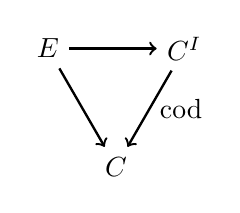
\begin{tikzpicture}[line width=0.3mm, scale=1]
              \node(e) at (150:1) {$E$}; 
              \node(ci) at (30:1) {$C^I$}; 
              \node(c) at (270:1) {$C$}; 
          
              \draw[->] (e) edge (ci)
                        (e) edge (c);
              \draw[->] (ci) edge node[right] {cod} (c);
            \end{tikzpicture}
        \end{center}
        where C I is the arrow category of C and cod:C I→C denotes the codomain projection (which is a fibration if C has pullbacks), and such that

    E→C is a Grothendieck fibration,

    E→C I takes cartesian morphisms in E to cartesian morphisms in C I (i.e. to pullback squares in C).
    \end{frame}
    \begin{frame}
        \frametitle{Category with families}
        A category with attributes specifies for each “context” only a set of “types” in that context. A comprehension category, by contrast, specifies a whole category of “types” in each context. If $A,B \in E \Gamma$, then we may think of a morphism $f:E\to A$ in $E \Gamma$ as a term in type theory.
        A category with families specifies instead, for each context and each type in that context, a set of “terms belonging to that type”. These should be thought of as terms in type theory.
    \end{frame}
    \section{Martin-Lof type theory}
    \subsection{Properties}
    \begin{frame}
        \frametitle{Martin-Lof type theory: Axiom of choice}
        \underline{Logical form of the axiom of choice:}\\
        Let $\sigma, \tau, \upsilon$ three types such that:
        $$\frac{}{\vdash \sigma \typ}\quad\frac{\vdash x:\sigma}{x:\sigma\vdash\tau\typ}\quad\frac{\vdash x:\sigma\quad \vdash y:\tau}{x:\sigma,y:\tau\vdash\upsilon\typ}$$
        \underline{Axiom of choice:}
        $$(\forall x : \sigma) (\exists y : \tau) \upsilon \to (\exists f : (\Pi x : \sigma)\tau)(\forall x : \sigma) \upsilon$$
    \end{frame}
    \subsection{Intensional and Extensional type theory}
    \begin{frame}
        \frametitle{Intensional and Extensional type theory}
        \begin{itemize}
            \item type theory + identity types = intensional type theory
            \item equality reflection:
            $$\frac{\Gamma \vdash M = N : \sigma}{\Gamma \vdash P: \Id{M}{N}}$$
            \item type theory + identity types + reflection rule = extensional type theory
            \item Judgmental equality and typing undecidable
        \end{itemize}
    \end{frame}
\end{document}